\documentclass[border=10pt]{standalone}
\usepackage{mathptmx}
\usepackage{amsmath,bm}
\usepackage{tikz}
\usetikzlibrary{arrows.meta,positioning,fit,calc,backgrounds}
\definecolor{gdark}{HTML}{5E7B5F}
\definecolor{glight}{HTML}{E6E9E4}
\definecolor{gbord}{HTML}{4A634B}
\definecolor{rloss}{HTML}{A8323E}
\definecolor{rsoft}{HTML}{F3DCDD}
\definecolor{note}{HTML}{F4F1E8}
\tikzset{
  dk/.style={draw=gbord,fill=gdark,text=white,rounded corners=3pt,align=center,font=\small,minimum height=12mm,minimum width=30mm,inner sep=5pt},
  lt/.style={draw=gray!60,fill=glight,text=black,rounded corners=3pt,align=center,font=\small,minimum height=12mm,minimum width=30mm,inner sep=5pt},
  ls/.style={draw=rloss,fill=rsoft,text=black,rounded corners=3pt,align=center,font=\small,minimum height=12mm,minimum width=30mm,inner sep=5pt,line width=0.8pt},
  nt/.style={draw=gray!50,fill=note,text=black!80,rounded corners=3pt,align=left,font=\footnotesize,inner sep=6pt},
  ar/.style={-{Stealth[length=2.6mm]},line width=0.8pt,draw=black!75},
  ard/.style={-{Stealth[length=2.6mm]},line width=0.8pt,draw=rloss,dashed},
  lb/.style={font=\footnotesize\itshape,text=black!70,align=center},
  frame/.style={draw=gbord,rounded corners=6pt,dashed,line width=0.7pt,inner sep=8pt},
  ttl/.style={font=\large\bfseries,text=black}
}
\newcommand{\x}{\bm{x}}

\begin{document}
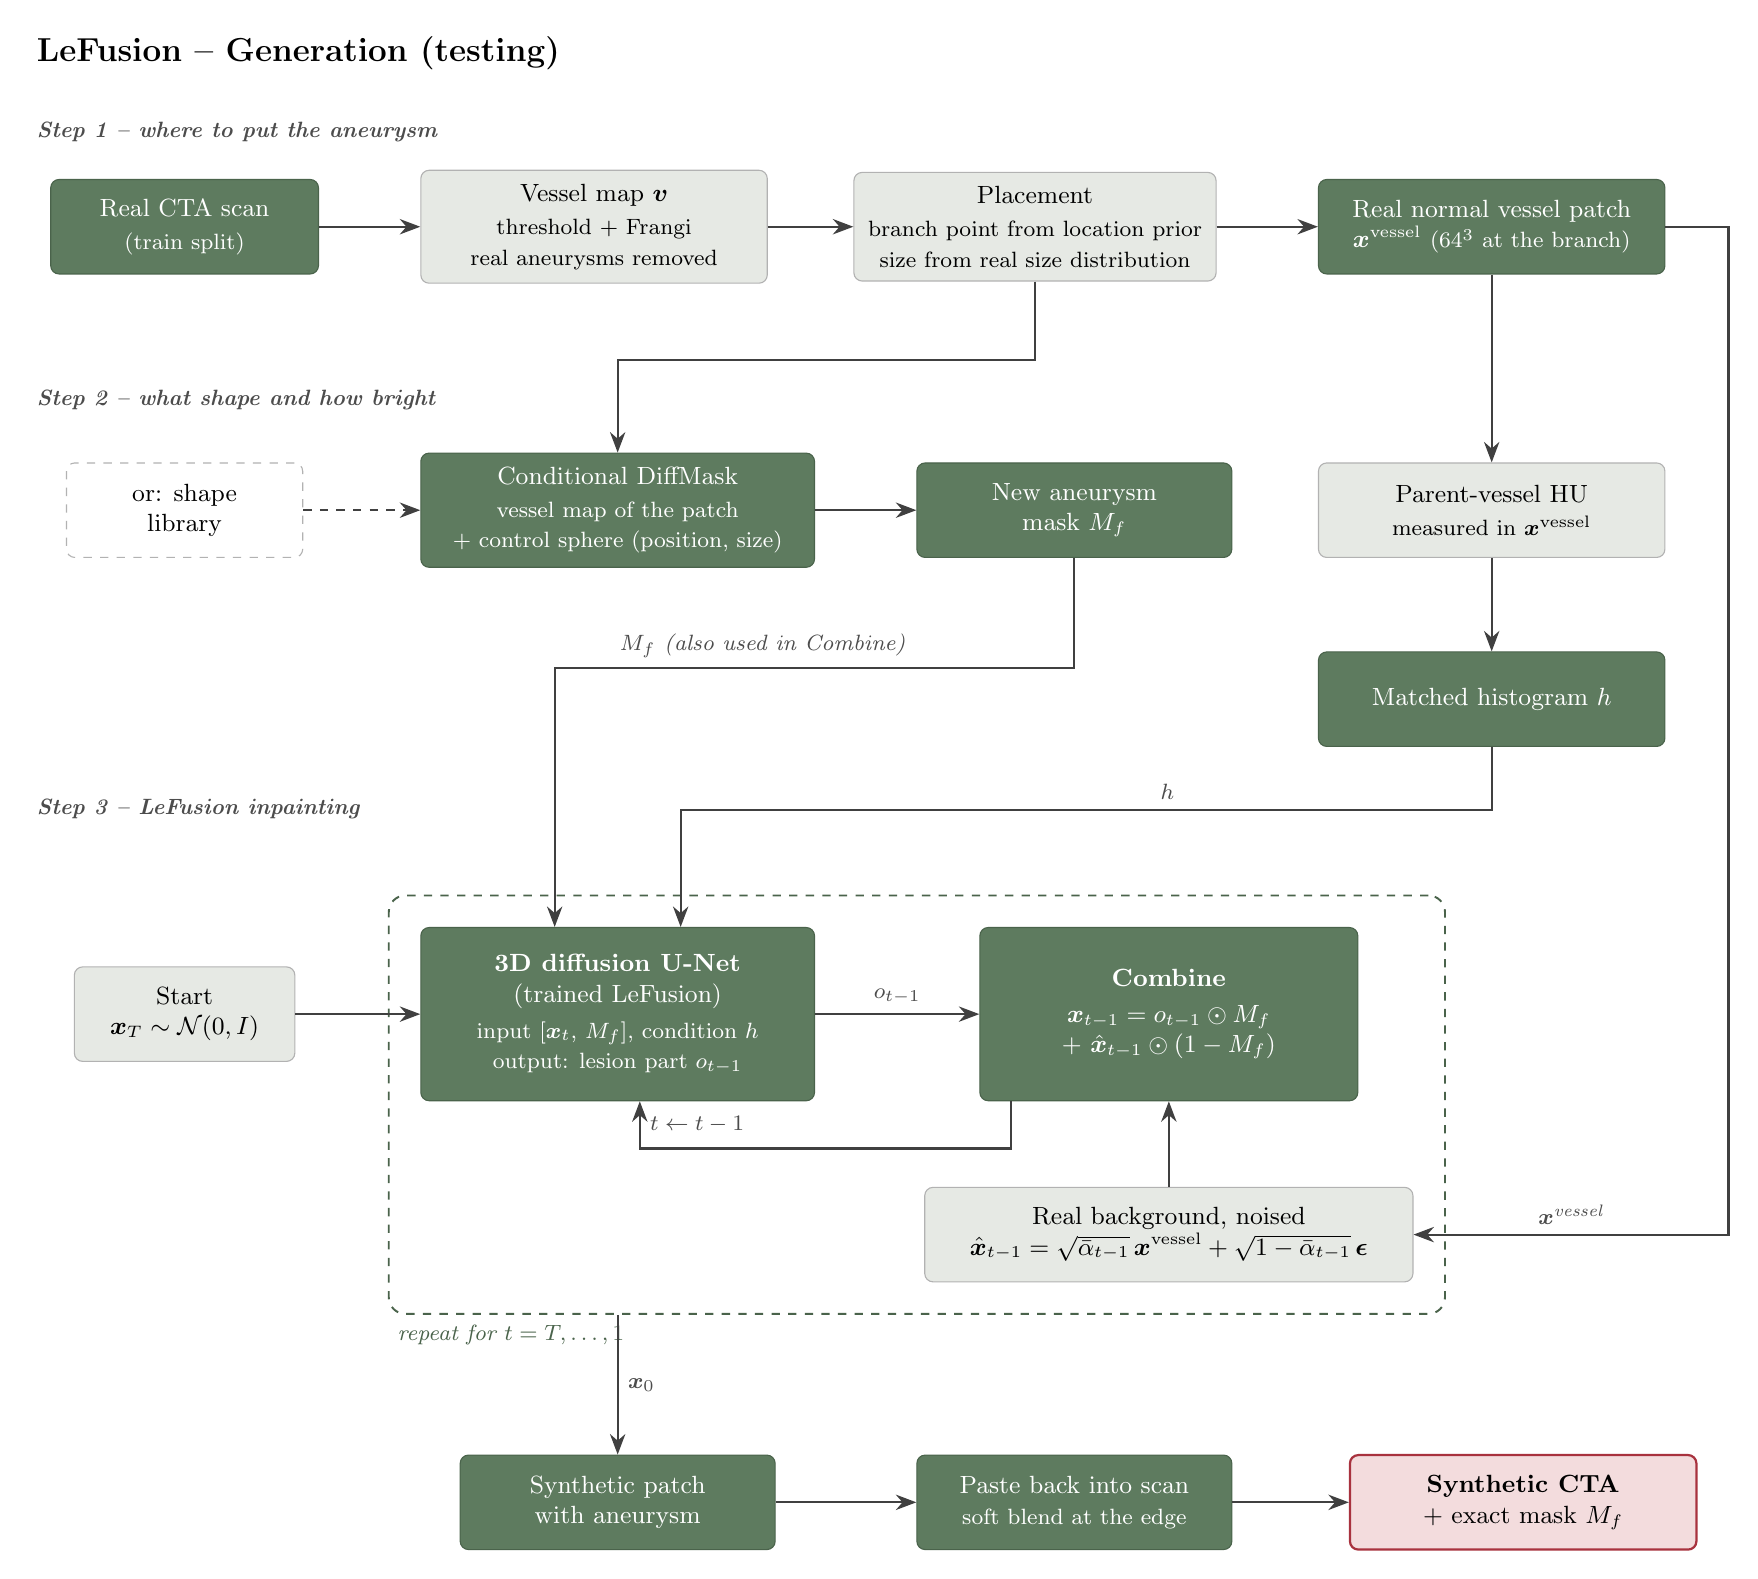
\begin{tikzpicture}[x=1mm,y=1mm]
% ---------- Step 1 ----------
\node[ttl, anchor=west] at (-20,22) {LeFusion -- Generation (testing)};
\node[lb, anchor=west] at (-20,12) {\bfseries Step 1 -- where to put the aneurysm};
\node[dk, minimum width=34mm] (scan) at (0,0) {Real CTA scan\\[1pt]\footnotesize (train split)};
\node[lt, minimum width=44mm] (ves) at (52,0) {Vessel map $\bm v$\\[1pt]\footnotesize threshold + Frangi\\\footnotesize real aneurysms removed};
\node[lt, minimum width=46mm] (plc) at (108,0) {Placement\\[1pt]\footnotesize branch point from location prior\\\footnotesize size from real size distribution};
\node[dk, minimum width=44mm] (vp) at (166,0) {Real normal vessel patch\\$\x^{\text{vessel}}$ \footnotesize ($64^3$ at the branch)};
\draw[ar] (scan)--(ves); \draw[ar] (ves)--(plc); \draw[ar] (plc)--(vp);

% ---------- Step 2 ----------
\node[lb, anchor=west] at (-20,-22) {\bfseries Step 2 -- what shape and how bright};
\node[lt, minimum width=30mm, fill=white, dashed] (lib) at (0,-36) {or: shape\\library};
\node[dk, minimum width=50mm] (dm) at (55,-36) {Conditional DiffMask\\[1pt]\footnotesize vessel map of the patch\\\footnotesize + control sphere (position, size)};
\node[dk, minimum width=40mm] (mf) at (113,-36) {New aneurysm\\mask $M_f$};
\node[lt, minimum width=44mm] (hu) at (166,-36) {Parent-vessel HU\\[1pt]\footnotesize measured in $\x^{\text{vessel}}$};
\node[dk, minimum width=44mm] (h) at (166,-60) {Matched histogram $h$};
\draw[ar] (plc.south) -- ++(0,-10) -| (dm.north);
\draw[ar, dashed] (lib)--(dm);
\draw[ar] (dm)--(mf);
\draw[ar] (vp)--(hu); \draw[ar] (hu)--(h);

% ---------- Step 3 ----------
\node[lb, anchor=west] at (-20,-74) {\bfseries Step 3 -- LeFusion inpainting};
\node[lt, minimum width=28mm] (xT) at (0,-100) {Start\\$\x_T\sim\mathcal N(0,I)$};
\node[dk, minimum width=50mm, minimum height=22mm] (u) at (55,-100) {\textbf{3D diffusion U-Net}\\(trained LeFusion)\\[2pt]\footnotesize input $[\x_t,\,M_f]$, condition $h$\\\footnotesize output: lesion part $o_{t-1}$};
\node[dk, minimum width=48mm, minimum height=22mm] (cb) at (125,-100) {\textbf{Combine}\\[2pt]$\x_{t-1}=o_{t-1}\odot M_f$\\$+\ \hat\x_{t-1}\odot(1-M_f)$};
\node[lt, minimum width=62mm] (bg) at (125,-128) {Real background, noised\\$\hat\x_{t-1}=\sqrt{\bar\alpha_{t-1}}\,\x^{\text{vessel}}+\sqrt{1-\bar\alpha_{t-1}}\,\bm\epsilon$};
\draw[ar] (xT)--(u);
\draw[ar] (u)--node[lb,above]{$o_{t-1}$}(cb);
\draw[ar] (bg)--(cb);
\draw[ar] (cb.south west) ++(4,0) |- ++(0,-6) -| node[lb,pos=0.75,right]{$t\leftarrow t-1$} ([xshift=8]u.south);
\begin{scope}[on background layer]
\node[frame, fit=(u)(cb)(bg), inner sep=4mm] (loop) {};
\end{scope}
\node[lb, anchor=north west, text=gbord] at (loop.south west) {repeat for $t=T,\dots,1$};
% inputs into the loop
\draw[ar] (mf.south) -- ++(0,-14) -| node[lb,pos=0.3,above]{$M_f$ (also used in Combine)} ([xshift=-8mm]u.north);
\draw[ar] (h.south) -- ++(0,-8) -| node[lb,pos=0.2,above]{$h$} ([xshift=8mm]u.north);
\draw[ar] (vp.east) -- ++(8,0) |- node[lb,pos=0.75,above]{$\x^{\text{vessel}}$} (bg.east);

% ---------- Output ----------
\node[dk, minimum width=40mm] (out) at (55,-162) {Synthetic patch\\with aneurysm};
\node[dk, minimum width=40mm] (paste) at (113,-162) {Paste back into scan\\\footnotesize soft blend at the edge};
\node[ls, minimum width=44mm] (fin) at (170,-162) {\textbf{Synthetic CTA}\\+ exact mask $M_f$};
\draw[ar] (loop.south -| out) -- node[lb,right]{$\x_0$} (out);
\draw[ar] (out)--(paste); \draw[ar] (paste)--(fin);
\end{tikzpicture}
\end{document}
